% !TeX root = ../main.tex

\chapter{Platform Design}\label{chapter:platform-design}

\section{Platform Design}
\label{sec:platform_design}

We design an aerodynamic surface-enhanced quadrotor in an X-wing configuration to preserve the agility of a conventional multirotor while benefiting from passive lift in forward flight.  
The design objective was to create a platform that remains fully compatible with existing quadrotor control architectures while achieving improved aerodynamic efficiency in the moderate-speed regime of \SIrange{5}{15}{\meter\per\second}.  
This range was chosen to match the operational envelope of modern visual–inertial odometry and path-planning algorithms, which rely on sufficient feature persistence and computation time when traversing complex environments.  
The platform maintains full hover capability and allows seamless transition between flight regimes, including the ability to come to a complete stop in the case of unexpected obstacles or path-planning delays.

\subsection{Configuration and Layout}

The overall configuration follows a conventional X-shaped quadrotor layout in which each rotor arm is extended into a fixed aerodynamic lifting surface, forming an ``X-wing'' planform.  
This choice leverages the inherent structural arrangement of a quadrotor—four arms symmetrically distributed around the center of gravity—while enabling these arms to generate lift instead of purely supporting the motors.  
Alternative configurations such as a ``plus'' (\(+\)) layout or biplane arrangements were considered less favorable:  
in a \(+\) configuration, two wings would be vertically oriented and thus unable to generate lift, while a biplane would require additional structural connections between the upper and lower planes, adding mass and complexity.  
The X-wing approach allows a single compact central frame with minimal added mass.

Each of the four wings has a span of \SI{0.45}{\meter} and a chord of \SI{0.25}{\meter}, resulting in an aspect ratio of approximately 1.8.  
The wing span was chosen to accommodate readily available \SI{0.5}{\meter} carbon rods used as internal spars, simplifying construction while placing the platform in the target cruise speed range of approximately \SI{10}{\meter\per\second}, where full aerodynamic lift would support the vehicle weight.  
The chord length was constrained by the available 3D printer build volume of just over \SI{250}{\milli\meter}; longer chords would have exceeded printability limits.  
The motor mounting legs, which position the motors in front of the wings and provide landing feet to avoid landing directly on the wing trailing edges, were printed diagonally within the build volume, further informing the final chord dimension.  
This value provides a balance between aerodynamic efficiency and structural stiffness; higher aspect ratios would improve lift–drag performance but increase bending inertia and reduce agility.  
The total diagonal motor-to-motor distance is \SI{1.1}{\meter}.  
All wings are mounted with alternating dihedral and anhedral angles of \(\pm \SI{45}{\degree}\), creating a fully symmetric configuration independent of flight direction.  
This symmetry enables the same controller gains to be used in roll and pitch and allows the yaw heading to be freely adjusted depending on which orientation minimizes control effort.

The wings are untwisted and employ a NACA~0015 symmetric airfoil.  
The choice of a symmetric section was motivated by the requirement for bidirectional flight and simple aerodynamic modeling.  
The thickness ratio of 15\% conveniently accommodates the two internal carbon spars used for stiffness and assembly.  
The NACA~0015 profile also exhibits a delayed stall and smooth lift curve, beneficial during transition and moderate-angle flight conditions.  
The chord line of each wing is aligned with the average rotor thrust axis (noting that the motors are tilted \(\pm\SI{5}{\degree}\) for yaw authority, as discussed below), such that the average motor thrust is directed vertically downward in hover without inducing horizontal force components.  
This alignment prioritizes hover efficiency, though tilting the wings relative to the motor thrust could improve forward-flight performance by allowing the motors to contribute a greater vertical component while the wings operate at reduced angles of attack.

The wings are printed from PLA~Aero filament and contribute a total of approximately \SI{440}{\gram} to the vehicle mass.  
All non-propulsive components (flight controller, companion computer, and batteries) are mounted near the geometric center, at \(x=y=0\), distributed symmetrically about the \(z=0\) plane to ensure balanced inertia.  
The complete airframe, including center hub and motor mounts, is fully 3D-printed.  
No structural asymmetries or significant vibrations were observed during geometric control experiments.  
However, when using the INDI controller, elastic wing vibrations appeared in the IMU data.  
To mitigate this, thin lines were tensioned between neighboring wings to increase stiffness and shift the dominant resonance frequency upward, improving signal filtering and control stability.

\subsection{Wing Structure and Manufacturing}

The wings were designed for additive manufacturing using fused deposition modeling (FDM) with PLA~Aero filament, which provides a favorable balance between low density, printability, and structural integrity.
Each wing features a hollow internal structure optimized to minimize mass while maintaining sufficient bending stiffness.

\paragraph{Internal structure.}
Figure~\ref{fig:wing_structure} shows the internal geometry of a single wing.
The NACA~0015 airfoil shell provides aerodynamic smoothness while keeping the structural mass low through a hollow internal cavity.
Internal ribs and supports are arranged to transfer loads from the aerodynamic surface to two parallel carbon fiber spars running spanwise through the wing.
The hollow core reduces the wing mass significantly compared to a solid print while providing channels for the \SI{10}{\milli\meter} diameter carbon spars that contribute the majority of the bending stiffness.
Each wing consists of two printed sections totaling approximately \SI{130}{\gram}, reinforced by two carbon fiber spars at approximately \SI{23}{\gram} each, resulting in a total wing mass of approximately \SI{176}{\gram} per wing.
This hybrid design—3D-printed aerodynamic shell with carbon reinforcement—achieves a favorable strength-to-weight ratio essential for minimizing inertia while maintaining structural integrity.

\paragraph{Manufacturing and assembly.}
Each wing is printed using vase mode (spiralize outer contour), which produces a single continuous spiral wall without retractions throughout the print.
This approach is particularly effective with PLA~Aero filament, which exhibits foaming behavior that leads to poor retraction performance and excessive stringing in conventional printing modes.
By eliminating retractions entirely, vase mode produces a clean, smooth aerodynamic surface with consistent wall thickness.
The wings are sliced and oriented vertically in the build volume to align the continuous spiral with the spanwise direction.
The two carbon spars are clamped into the printed channels using a central core structure, eliminating the need for adhesives and enabling rapid part replacement for testing and repair.
The motor mounting legs and landing feet are printed separately using conventional settings and mechanically attached to the wing structure.

Each wing is capped with an endcap component (Figure~\ref{fig:wing_foot}) that serves multiple functions: it closes the hollow wing structure, provides mounting points for the motors positioned ahead of the leading edge, and extends downward to form landing feet that protect the wing trailing edges during ground contact.
This integrated design consolidates three separate functions into a single 3D-printed part, simplifying assembly and reducing the total part count.
The motor mounting angle includes a \(\pm\SI{5}{\degree}\) tilt to enable differential thrust for yaw control.

The central core (Figure~\ref{fig:core_structure}) serves as the primary structural hub that clamps all carbon spars and houses the critical electronics.
Two identical cores are used: one for the four upper spars and one for the four lower spars.
This identical design simplifies manufacturing and allows the same printed part to be used for both top and bottom assemblies.
The top core houses the electronic speed controllers (ESC), flight controller (FC), and batteries, positioning them near the center of mass for optimal weight distribution, while the bottom core serves purely as a structural clamp for the lower spars.
A snap-on lid covers the top core, providing additional structural stiffness, protecting the electronics, and forming a flat mounting base for the batteries.
This modular clamping architecture allows individual wings or carbon spars to be quickly exchanged without disassembly of the entire airframe.

\begin{figure}[htbp]
\centering
\includegraphics[width=0.48\linewidth]{figures/wing_transparent.png}
\hfill
\includegraphics[width=0.48\linewidth]{figures/wing_sliced.png}
\caption{Wing structure and manufacturing: (left) CAD model showing the hollow internal geometry with channels for carbon fiber spars, (right) sliced preview in vase mode showing the continuous spiral toolpath that eliminates retractions and produces a clean aerodynamic surface.}
\label{fig:wing_structure}
\end{figure}

\begin{figure}[htbp]
\centering
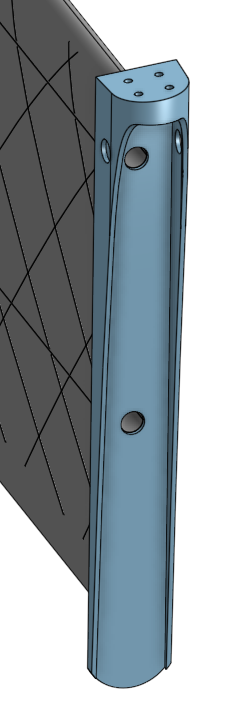
\includegraphics[height=0.4\linewidth]{figures/foot.png}
\caption{Wing endcap component serving as motor mount and landing foot. This multi-functional part closes the hollow wing structure, positions the motor ahead of the leading edge with a \(\pm\SI{5}{\degree}\) tilt for yaw control, and extends downward to protect the wing trailing edge during landing.}
\label{fig:wing_foot}
\end{figure}

\begin{figure}[htbp]
\centering
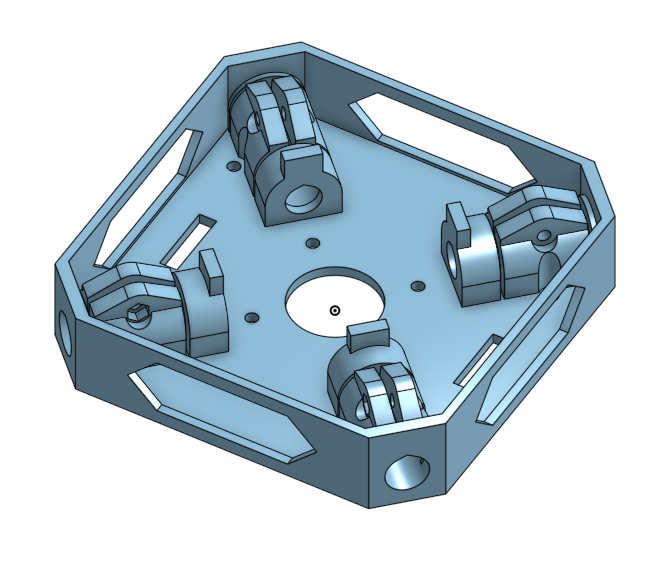
\includegraphics[width=0.6\linewidth]{figures/core.png}
\caption{Central core structure that clamps the carbon fiber spars. Two identical cores are used for ease of manufacturing: one houses the ESC, flight controller, and batteries (top), while the other serves as a structural clamp for the lower spars (bottom). A snap-on lid (not shown) covers the top core for additional stiffness and battery mounting.}
\label{fig:core_structure}
\end{figure}

\subsection{Wing Aerodynamics}

The aerodynamic surfaces were designed for efficient lift generation in the cruise speed range of \SIrange{5}{15}{\meter\per\second}.  
At a nominal flight velocity of \SI{10}{\meter\per\second} and chord length of \SI{0.25}{\meter}, the expected Reynolds number is on the order of \(1\times10^5\)–\(2\times10^5\), placing the operation in the low-Reynolds transitional regime.

The Reynolds number characterizes the ratio of inertial to viscous forces and is computed as
\begin{equation}
Re = \frac{\rho V c}{\mu} = \frac{V c}{\nu},
\label{eq:reynolds_number}
\end{equation}
where \(\rho\) is the air density, \(V\) is the airspeed, \(c\) is the chord length, \(\mu\) is the dynamic viscosity, and \(\nu\) is the kinematic viscosity of air.
Using standard atmospheric conditions at sea level (\(\rho = 1.225~\mathrm{kg/m^3}\), \(\nu = 1.4207 \times 10^{-5}~\mathrm{m^2/s}\)) and the wing chord length of \(c = 0.25~\mathrm{m}\), the Reynolds number is approximately \(Re \approx 1.76 \times 10^5\) at \SI{10}{\meter\per\second} and \(Re \approx 5.27 \times 10^5\) at \SI{30}{\meter\per\second}.

At the \SI{10}{\meter\per\second} cruise condition (\(Re \approx 2 \times 10^5\)), the NACA~0015 profile achieves a lift coefficient of approximately \(C_L \approx 0.97\) at \(\alpha \approx 10^\circ\) and a drag coefficient of \(C_D \approx 0.025\).
The target angle of attack in steady cruise was set to around \SI{10}{\degree}.  
At this design cruise angle of attack, the airfoil provides sufficient lift to support the vehicle weight at moderate forward speeds.
A detailed comparison of the NACA~0015 baseline airfoil against an improved AG25 airfoil, including aerodynamic performance metrics and their correlation with flight test results, is presented in Chapter~\ref{chapter:experiments-evaluation}.

Lift and drag forces were estimated using the analytical model introduced earlier,
\[
L = \tfrac{1}{2} \rho S C_L(\alpha) \|v_a\|^2, \quad
D = \tfrac{1}{2} \rho S C_D(\alpha) \|v_a\|^2,
\]
with \(\rho\) denoting air density, \(S\) the total projected wing area, and \(v_a\) the airspeed relative to the body.  
These analytical estimates guided the sizing of the vehicle and the placement of the aerodynamic surfaces relative to the center of gravity.

\paragraph{Quantitative estimate at \(12~\mathrm{m/s}\).}
Using \(\rho=1.225~\mathrm{kg/m^3}\), total projected wing area \(S \approx 0.318~\mathrm{m^2}\), \(C_L \approx 0.97\) at \(\alpha \approx 10^\circ\), and \(C_D \approx 0.025\), we obtain
\[
L \;=\; \tfrac{1}{2}\,\rho\,S\,C_L\,V^2
\;\approx\; \tfrac{1}{2}\cdot 1.225 \cdot 0.318 \cdot 0.97 \cdot (12)^2
\;\approx\; 27.2~\mathrm{N},
\]
\[
D \;=\; \tfrac{1}{2}\,\rho\,S\,C_D\,V^2
\;\approx\; \tfrac{1}{2}\cdot 1.225 \cdot 0.318 \cdot 0.025 \cdot (12)^2
\;\approx\; 0.70~\mathrm{N}.
\]
For the \SI{2.5}{kg} platform (\(W \approx 24.53~\mathrm{N}\)), the wings supply \(\approx 111\%\) of the weight at \(12~\mathrm{m/s}\), meaning the rotors can reduce thrust significantly and primarily need to overcome aerodynamic drag and provide control authority. The wing-induced drag corresponds to \(\approx 8.4~\mathrm{W}\) of propulsive power at \(12~\mathrm{m/s}\) (\(P_D = D\,V\)), not accounting for additional parasite/induced drag from the fuselage, rotors, and interference effects. These values are first-order estimates based on XFLR5 analysis and neglect propeller–wing interaction; they nonetheless quantify the expected forward-flight relief on rotor-induced power.

Propeller–wing interaction effects were not explicitly studied in this work.  
Since the wings are aligned with the rotor arms, partial overlap between the propeller wake and wing surface occurs, but its contribution to performance is assumed to be secondary compared to the main aerodynamic lift of the forward wings.  
Future investigations could employ CFD or wind-tunnel testing to quantify this coupling.

\subsection{Propulsion and Actuation}

The propulsion system was designed to maintain high agility while achieving efficient cruise performance.  
A thrust-to-weight ratio exceeding 3 was selected as a design target, enabling the vehicle to perform aggressive maneuvers and sustain up to \SI{3}{g} lateral acceleration, consistent with agility metrics reported in the multirotor literature.  
To meet this target, high-response racing-grade components were chosen:  
T-MOTOR VELOX~V2808 motors combined with HQProp~7×3.5×3 three-blade propellers.  
The resulting hover throttle is approximately 30\%, leaving sufficient control margin for disturbance rejection and attitude stabilization.

Motor and propeller performance were characterized experimentally to obtain both thrust and torque mappings.  
The measurements were performed using a single motor mounted on a six-axis force–torque sensor, with forces and torques recorded over a range of command inputs.  
The empirical relations between motor command, thrust, and torque were used to map the controller outputs into corresponding DShot commands for the flight controller.  
These mappings also served to estimate instantaneous energy consumption and mechanical efficiency during flight trials.

The motors are tilted outward by \SI{5}{\degree} to increase effective yaw torque authority.  
In the control model, this tilt is represented as a small rotation of the individual thrust vectors, effectively increasing the available moment around the vertical axis.  
No DShot timing modifications were required, and no direct RPM feedback control was implemented.  
Instead, the INDI controller integrates motor speed responses and compensates for small deviations, ensuring smooth dynamic performance.

Although the addition of wings increases the total inertia of the platform, particularly in yaw, the resulting damping improved stability and reduced sensitivity to high-frequency disturbances.  
No significant cross-coupling between roll and pitch dynamics was observed.  
Overall, the X-wing configuration provides a good compromise between efficiency and agility, maintaining the control simplicity of a quadrotor while offering measurable lift benefits in forward flight.  
Performance gains were compared analytically against a non-winged reference quadrotor of comparable size and propulsion, confirming a theoretical reduction in power consumption at moderate forward velocities.

% TODO: Add figure
% \begin{figure}[h]
% \centering
% \includegraphics[width=0.8\linewidth]{figures/xwing_layout.pdf}
% \caption{X-wing aerodynamic surface-enhanced quadrotor layout showing the symmetric dihedral configuration and component arrangement.}
% \label{fig:xwing_layout}
% \end{figure}
